\documentclass[../AnalysisNoteJBuxton.tex]{subfiles}
\begin{document}

\subsubsection{\texorpdfstring{$\Lambda$}{TEXT} Reconstruction}
\label{LambdaReconstruction}

The following cuts were used to select good \LamALam candidates:

\begin{enumerate}
 \item Daughter Particle Cuts
 \begin{enumerate}
  \item{Cuts Common to Both Daughters}
  \begin{enumerate}
   \item $|\eta| < 0.8$
   \item SetTPCnclsDaughters(80)
   \item SetStatusDaughters(AliESDtrack::kTPCrefit)
   \item DCA $\pi$p Daughters $<$ 0.4 cm
  \end{enumerate}
  \item Pion Specific Daughter Cuts 
  \begin{enumerate}
   \item $p_{\mathrm{T}} > 0.16$ GeV/\textit{c}
   \item DCA to prim vertex $>$ 0.3 cm
   \item TPC and TOF N$\sigma$ Cuts
   \begin{enumerate}
    \item $p <$ 0.5 GeV/\textit{c} : N$\sigma_{\mathrm{TPC}} <$ 3
    \item $p >$ 0.5 GeV/\textit{c} :
    \begin{itemize}
     \item if TOF \& TPC available: N$\sigma_{\mathrm{TPC}} <$ 3 \& N$\sigma_{\mathrm{TOF}} <$ 3
     \item else N$\sigma_{\mathrm{TOF}} <$ 3
    \end{itemize}
   \end{enumerate}
  \end{enumerate}
  \item Proton Specific Daughter Cuts
  \begin{enumerate}
   \item $p_{\mathrm{T}} > $ 0.5($p$) [0.3($\bar{p}$)] GeV/\textit{c}
   \item DCA to prim vertex $>$ 0.1 cm
   \item TPC and TOF N$\sigma$ Cuts
   \begin{enumerate}
    \item $p <$ 0.8 GeV/\textit{c} : N$\sigma_{\mathrm{TPC}} <$ 3
    \item $p >$ 0.8 GeV/\textit{c} :
    \begin{itemize}
     \item if TOF \& TPC available: N$\sigma_{\mathrm{TPC}} <$ 3 \& N$\sigma_{\mathrm{TOF}} <$ 3
     \item else N$\sigma_{\mathrm{TOF}} <$ 3
    \end{itemize}
   \end{enumerate}   
  \end{enumerate}
 \end{enumerate}
 \item V0 Cuts
 \begin{enumerate}
  \item $|\eta| < 0.8$
  \item $p_{\mathrm{T}} > 0.4$ GeV/\textit{c}
  \item $|m_{\mathrm{inv}} - m_{\mathrm{PDG}}| <$ 3.8 MeV
  \item DCA to prim. vertex $<$ 0.5 cm
  \item Cosine of pointing angle $>$ 0.9993
  \item OnFlyStatus = false
  \item Decay Length $<$ 60 cm
 \end{enumerate}
 \item Shared Daughter Cut for V0 Collection
 \begin{itemize}
  \item Iterate through V0 collection to ensure that no daughter is used in more than one V0 candidate
 \end{itemize}
\end{enumerate} 


\begin{figure}[h!]
  \centering
  %%----start of first subfigure---  
  \subfloat[Mass assuming \Ks-hypothesis for \Lam collection, \newline i.e. assume the daughters are $\pi^{+}\pi^{-}$ instead of $p^{+}\pi^{-}$.]{
    \label{fig:MassAssK0ShortHyp_cLamK0:a}
    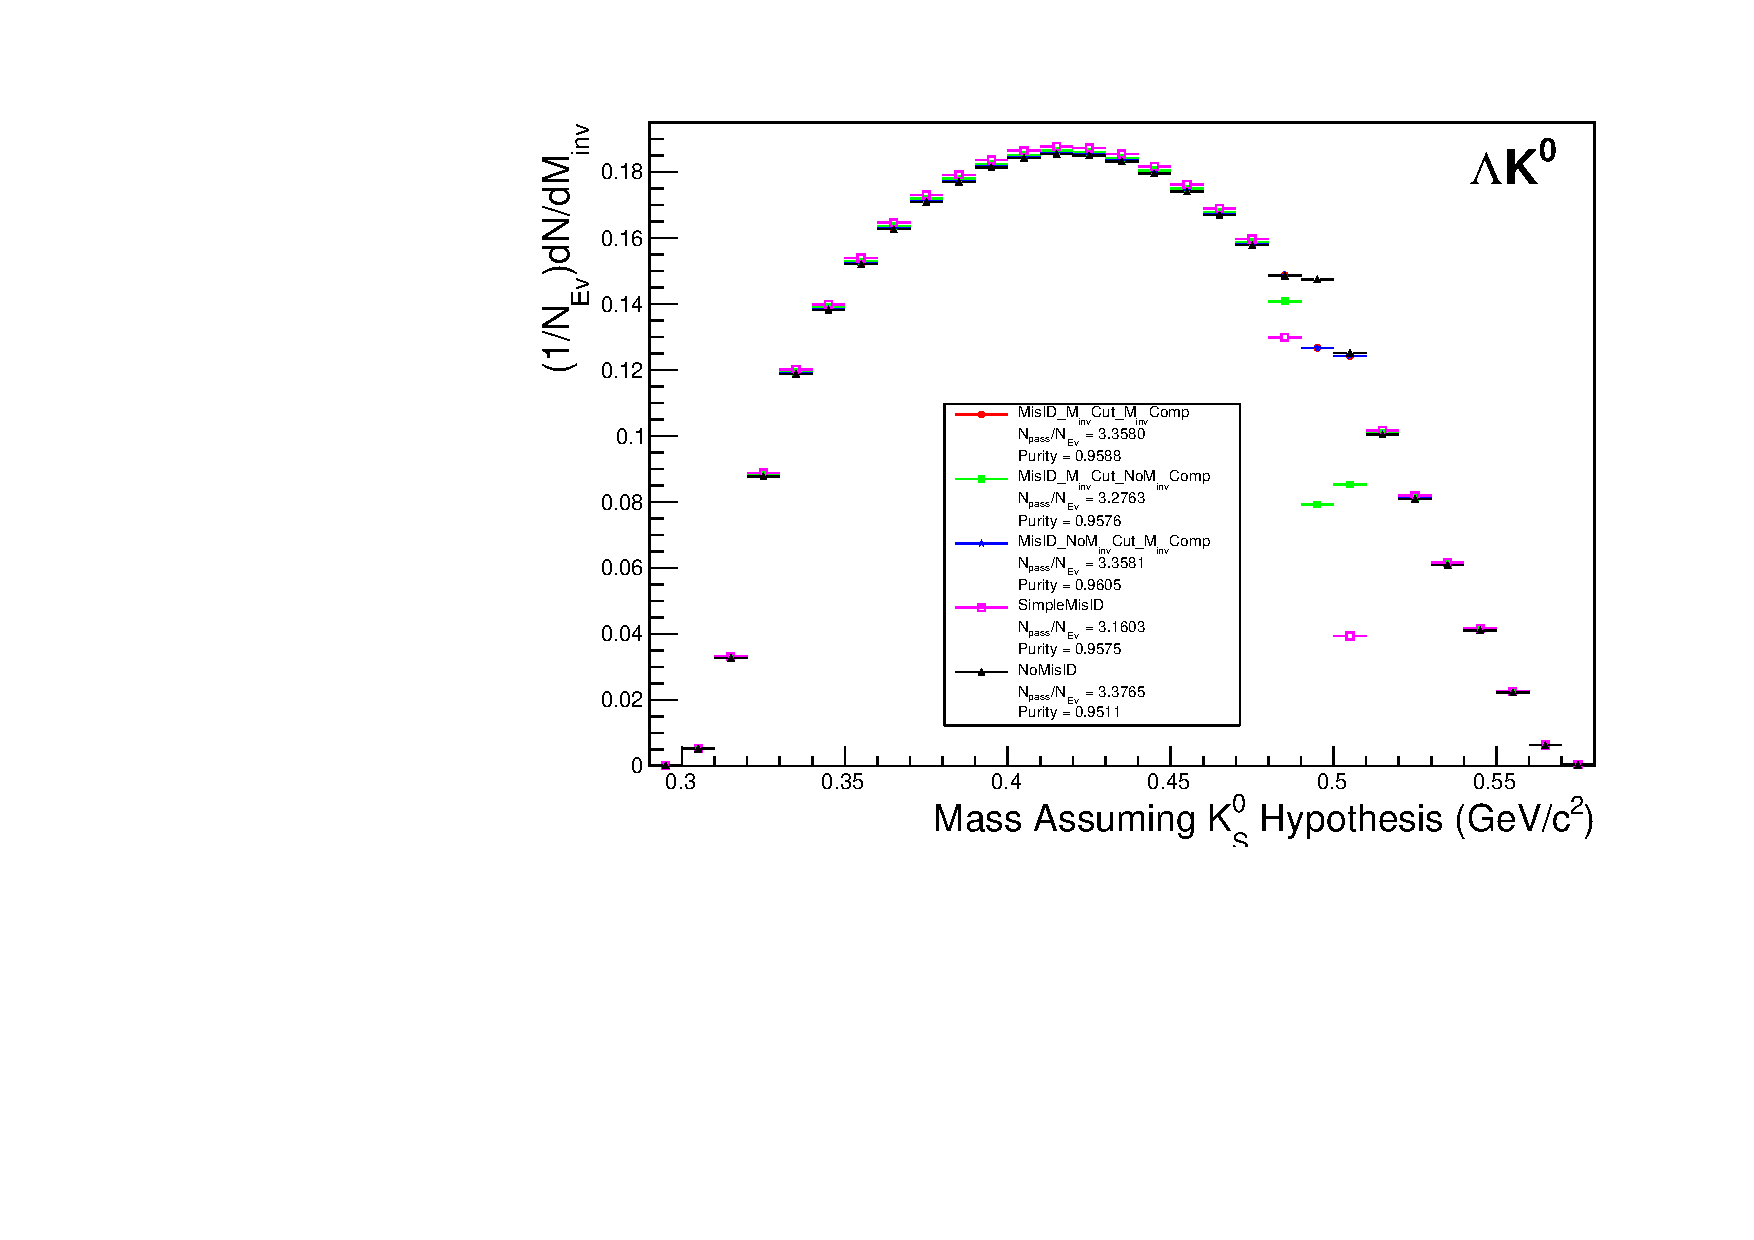
\includegraphics[width=0.49\textwidth]{3_DataSelection/Figures/MassAssHypotheses/canMassAssK0HypCompare_LamK0_wNoMisID.pdf}}%\\
  %%----start of second subfigure---
  \subfloat[Mass assuming \Ks-hypothesis for \ALam collection, \newline i.e. assume the daughters are $\pi^{+}\pi^{-}$ instead of $\pi^{+}\bar{p}^{-}$.]{
    \label{fig:MassAssK0ShortHyp_cLamK0:b}
    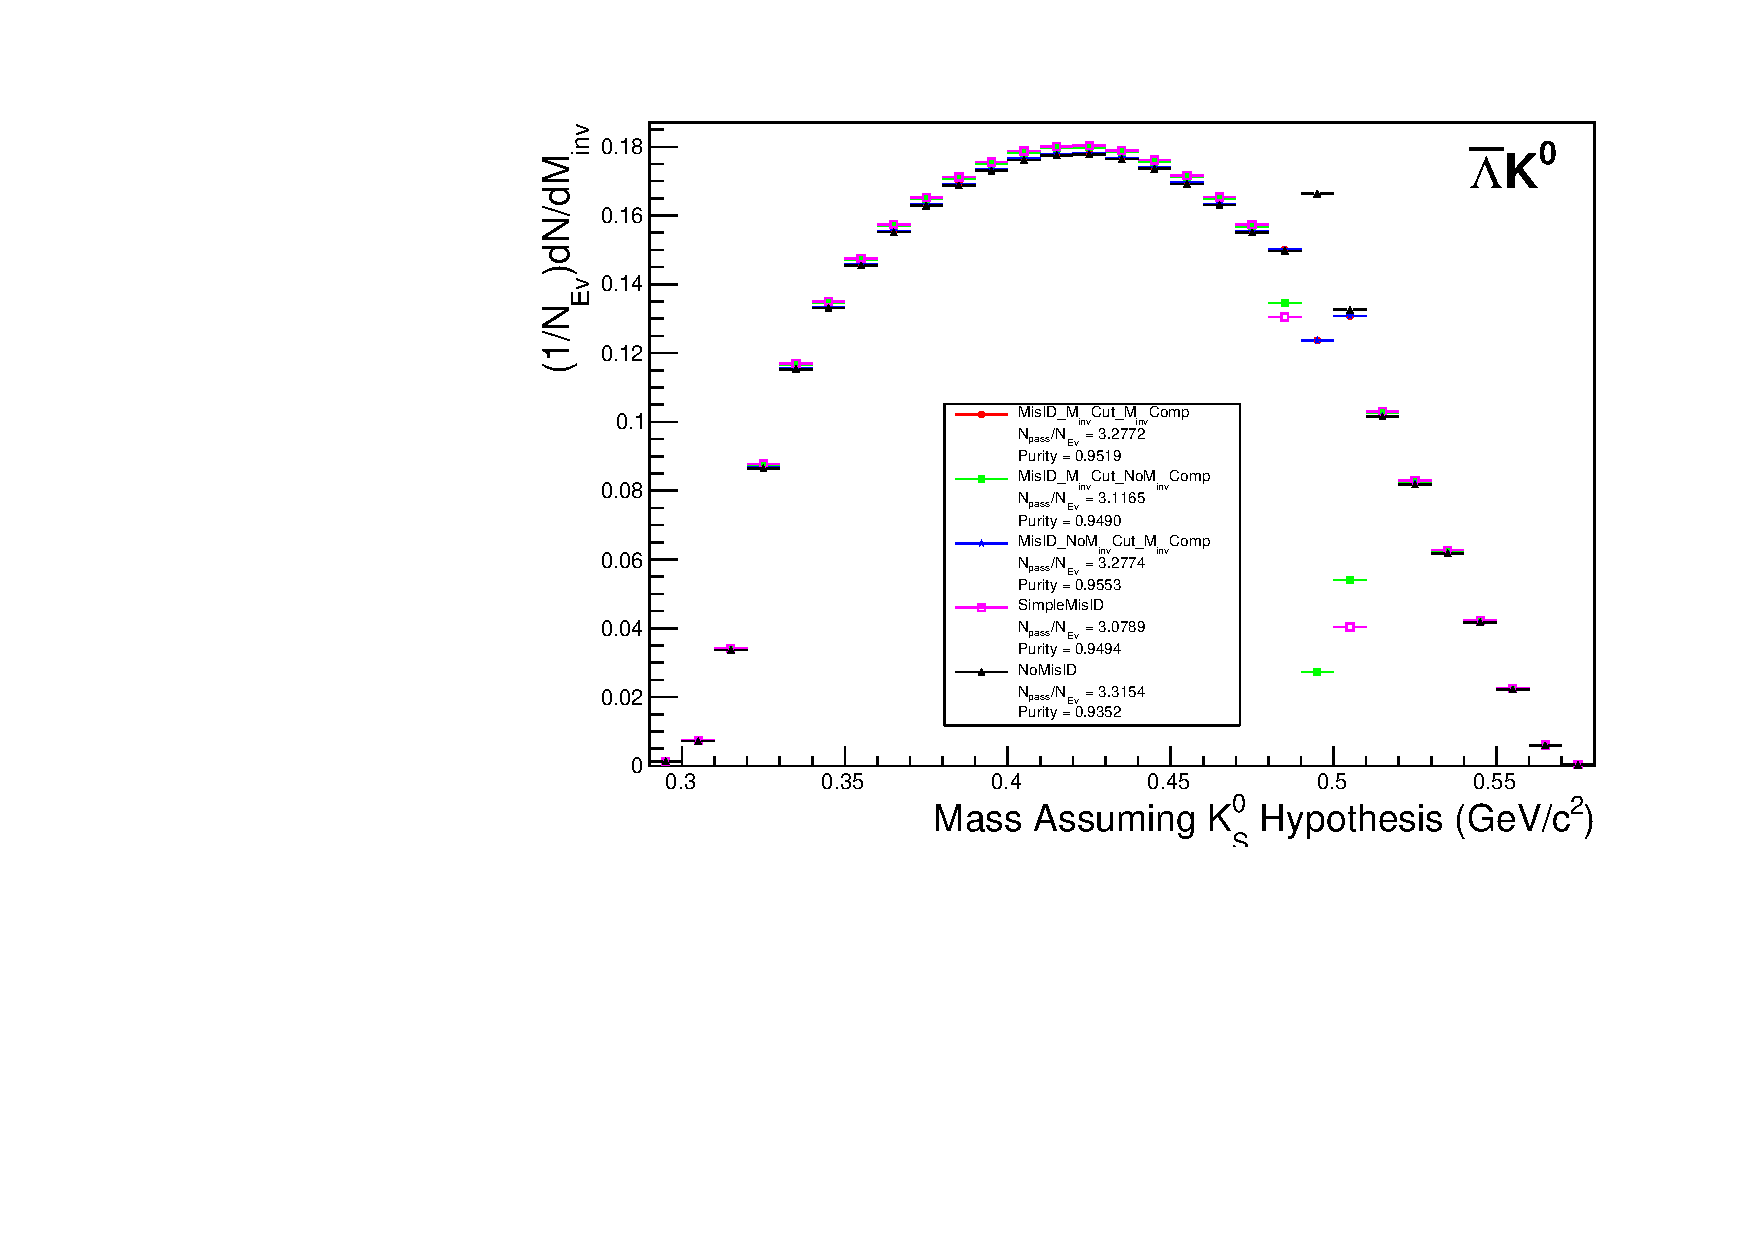
\includegraphics[width=0.49\textwidth]{3_DataSelection/Figures/MassAssHypotheses/canMassAssK0HypCompare_ALamK0_wNoMisID.pdf}}
  %%----overall caption----
  \caption[\Ks contamination in \LamALam collection]{Mass assuming \Ks-hypothesis for V0 candidates passing all \Lam (\ref{fig:MassAssK0ShortHyp_cLamK0:a}) and \ALam (\ref{fig:MassAssK0ShortHyp_cLamK0:b}) cuts.
  The ``NoMisID" distribution (black triangles) uses the V0 finder without any attempt to remove misidentified \Ks
  The slight peak in the ``NoMisID" distribution around $m_{\mathrm{inv}}$ = 0.5 GeV/$c^{2}$ contains misidentified \Ks particles in our \LamALam collection.  
  ``SimpleMisID" (pink squares) simply cuts out the entire peak, which throws away some good \Lam and \ALam particles.
  ``MisID\_NoM$_{\mathrm{inv}}$Comp" (green squares) uses the misidentification cut outlined in the text, but does not utilize the final invariant mass comparison step.
  ``MisID\_M$_{\mathrm{inv}}$Comp" (red circles) utilizes the full misidentification methods, and is currently used for this analysis.  
  ``N$_{pass}$/N$_{ev}$" is the total number of \LamALam particles found, normalized by the total number of events.  The purity of the collection is also listed.}
  \label{fig:MassAssK0ShortHyp_cLamK0}
\end{figure}

Figure \ref{fig:MassAssK0ShortHyp_cLamK0:a} shows the mass assuming \Ks hypothesis for the \Lam collection, i.e. assume the daughters are $\pi^{+}\pi^{-}$ instead of p$^{+}\pi^{-}$.
Figure \ref{fig:MassAssK0ShortHyp_cLamK0:b} is a similar plot, but is for the \ALam collection, i.e. assume the daughters are $\pi^{+}\pi^{-}$ instead of $\pi^{+}\bar{p}^{-}$.
The \Ks contamination is visible, although not profound, in both, in the slight peaks around $m_{\mathrm{inv}}$ = 0.497 GeV/$c^{2}$.
If one simply cuts out the entire peak, good \Lam particles will be lost.
Ideally, the \Lam selection and \Ks misidentification cuts are selected such that the peak is removed from this plot while leaving the underlying distribution continuous.
To attempt to remove these \Ks contaminations without throwing away good \Lam and \ALam particles, the following misidentification cuts are imposed; a \LamALam candidate is rejected if all of the following criteria are satisfied:
\begin{itemize}
 \item $\left|m_{\mathrm{inv,~ K^{0}_{S}~ Hypothesis}} - m_{\mathrm{PDG,~ K^{0}_{S}}}\right| < $ 9.0 MeV/$c^{2}$
 \item Positive and negative daughters pass $\pi$ daughter cut implemented for K$^{0}_{S}$ reconstruction
 \item $\left|m_{\mathrm{inv,~ K^{0}_{S}~ Hypothesis}} - m_{\mathrm{PDG,~ K^{0}_{S}}}\right|~ < ~\left|m_{\mathrm{inv,~ \Lambda(\bar{\Lambda})~ Hypothesis}} - m_{\mathrm{PDG,~ \Lambda(\bar{\Lambda})}}\right|$
\end{itemize} 


Figure \ref{fig:cLamPurity} shows the invariant mass (m$_{\mathrm{inv}}$) distribution of all $\Lambda$($\bar{\Lambda}$) candidates immediately before the final invariant mass cut.
These distributions are used to calculate the collection purities.
The $\Lambda$ and $\bar{\Lambda}$ purities are found to be: Purity($\Lambda$) $\approx$ Purity($\bar{\Lambda}$) $\approx$ 95\%.

\begin{figure}[h!]
  \centering
  %%----start of first subfigure---  
  \subfloat[$\Lambda$ Purity]{
    \label{fig:cLamPurity:a}
    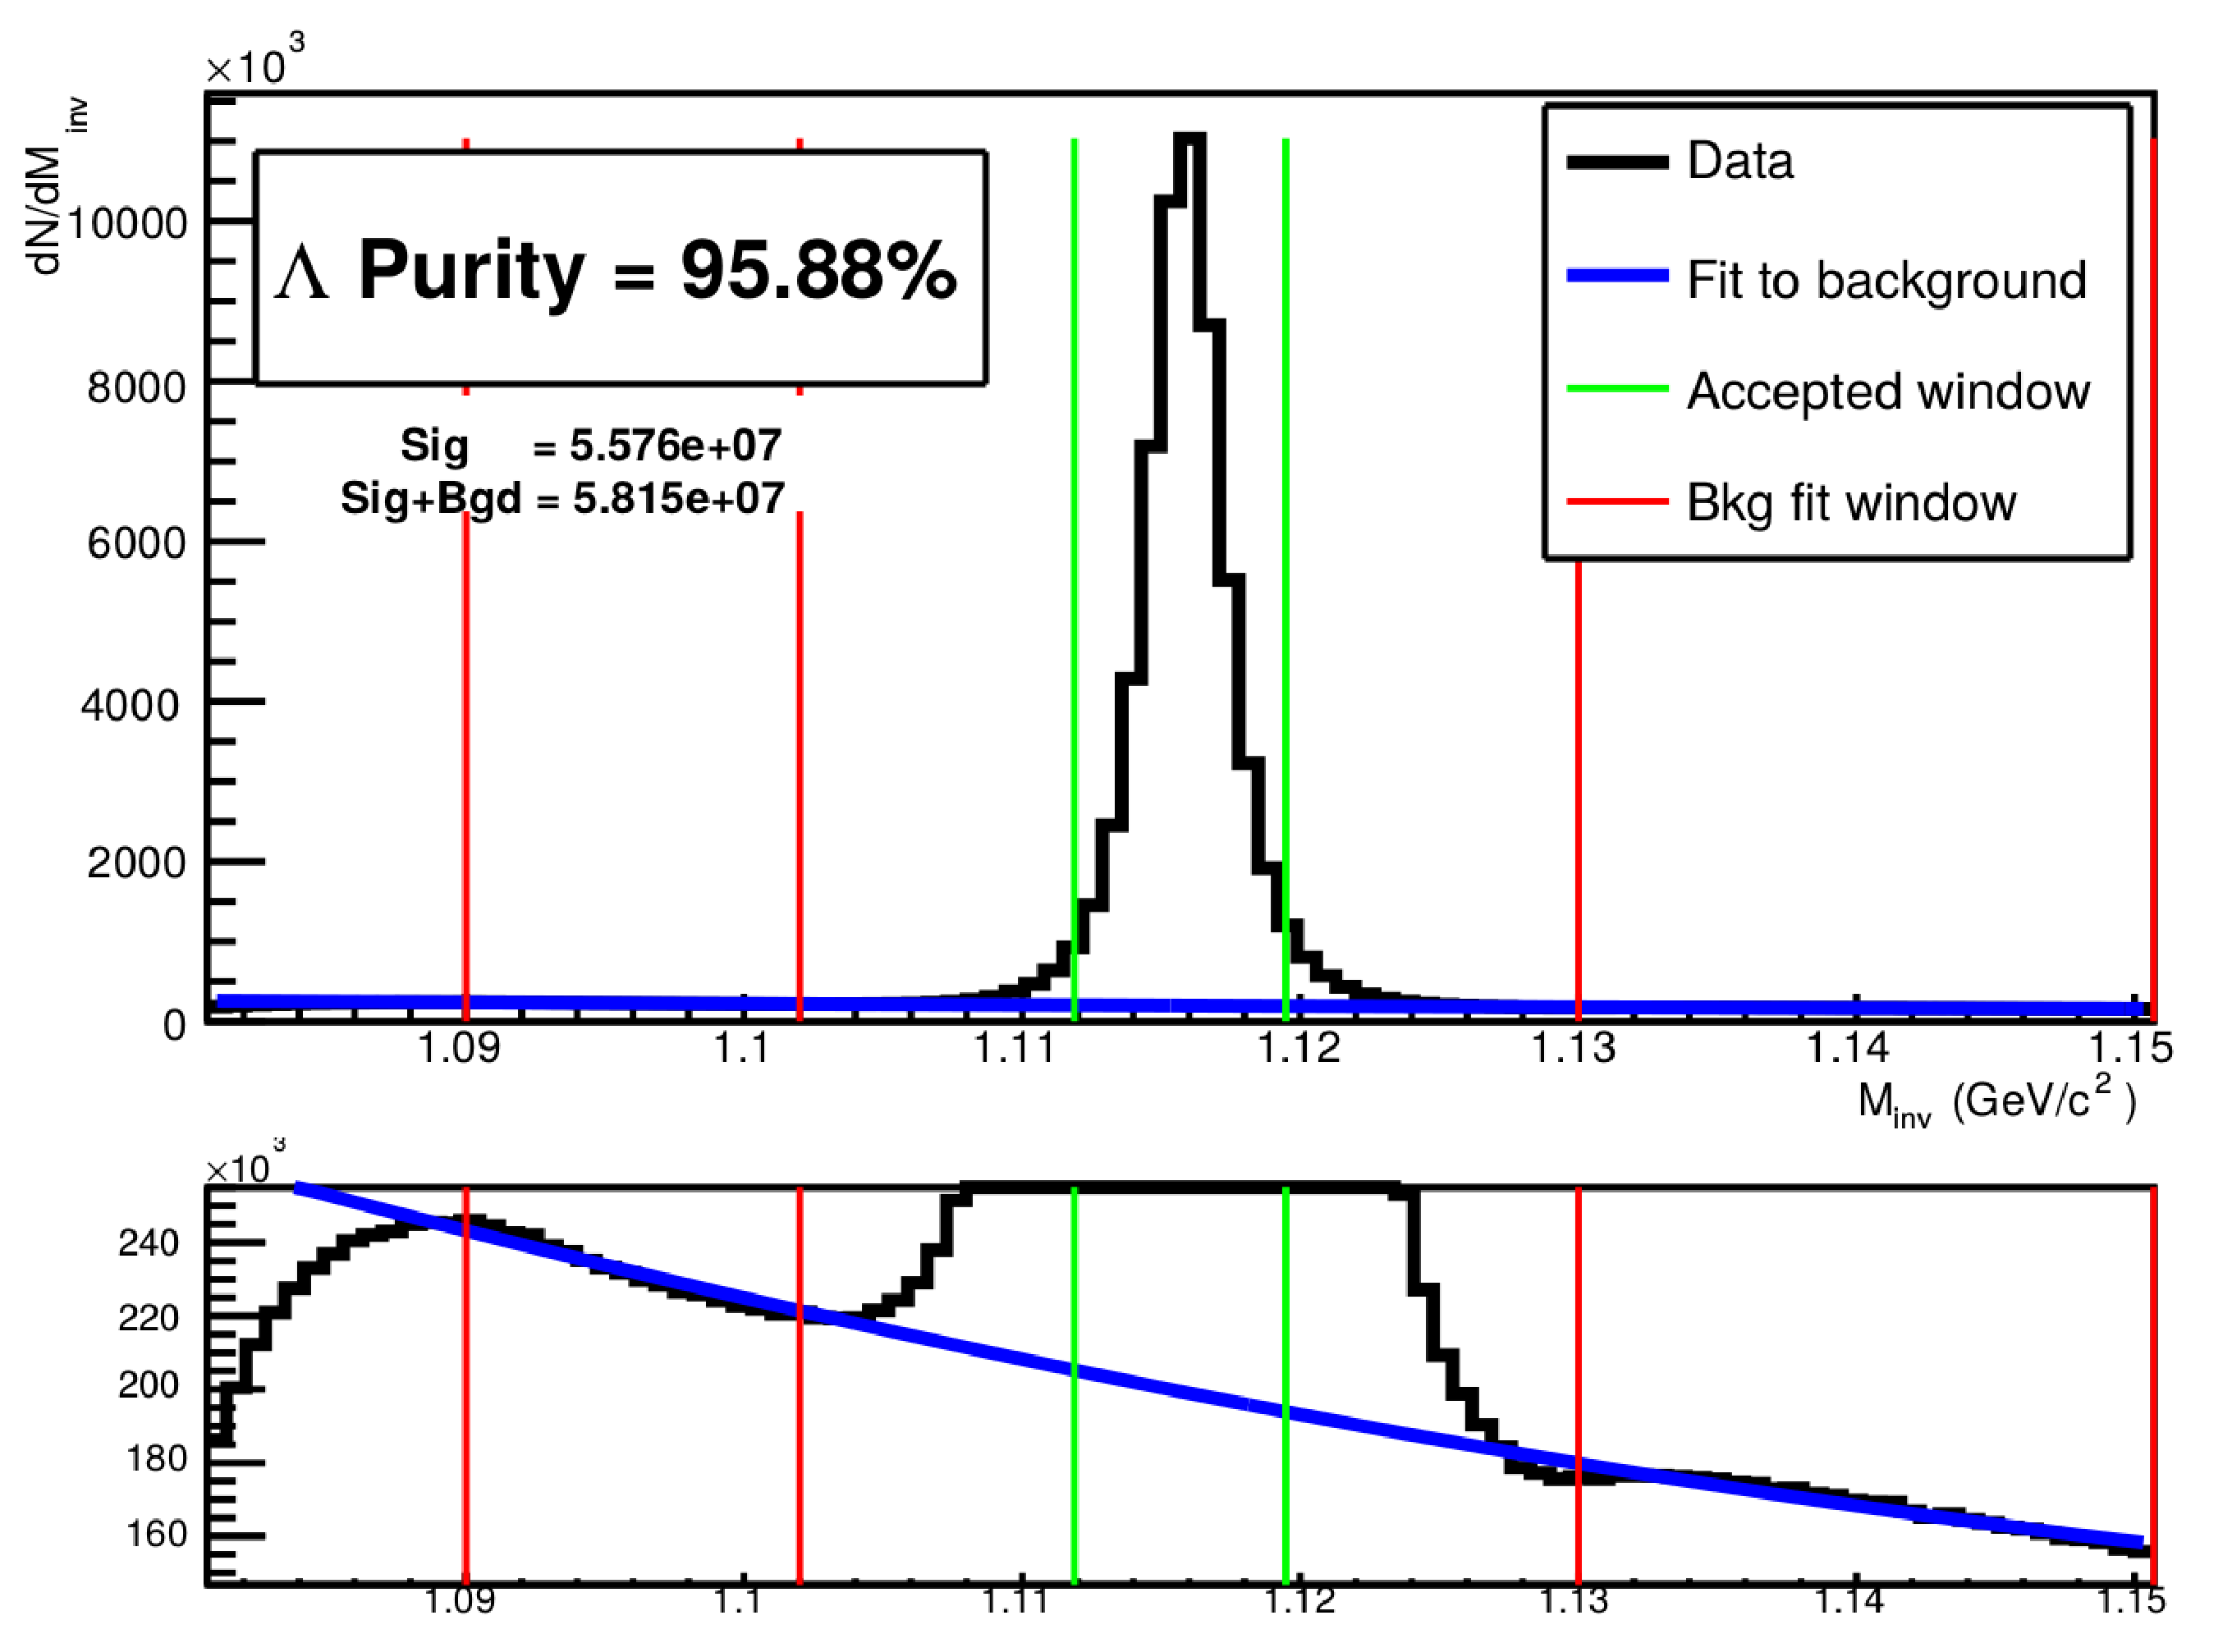
\includegraphics[width=0.49\textwidth]{3_DataSelection/Figures/LamPurity_LamKch_0010.pdf}}%\\
  %%----start of second subfigure---
  \subfloat[$\bar{\Lambda}$ Purity]{
    \label{fig:cLamPurity:b}
    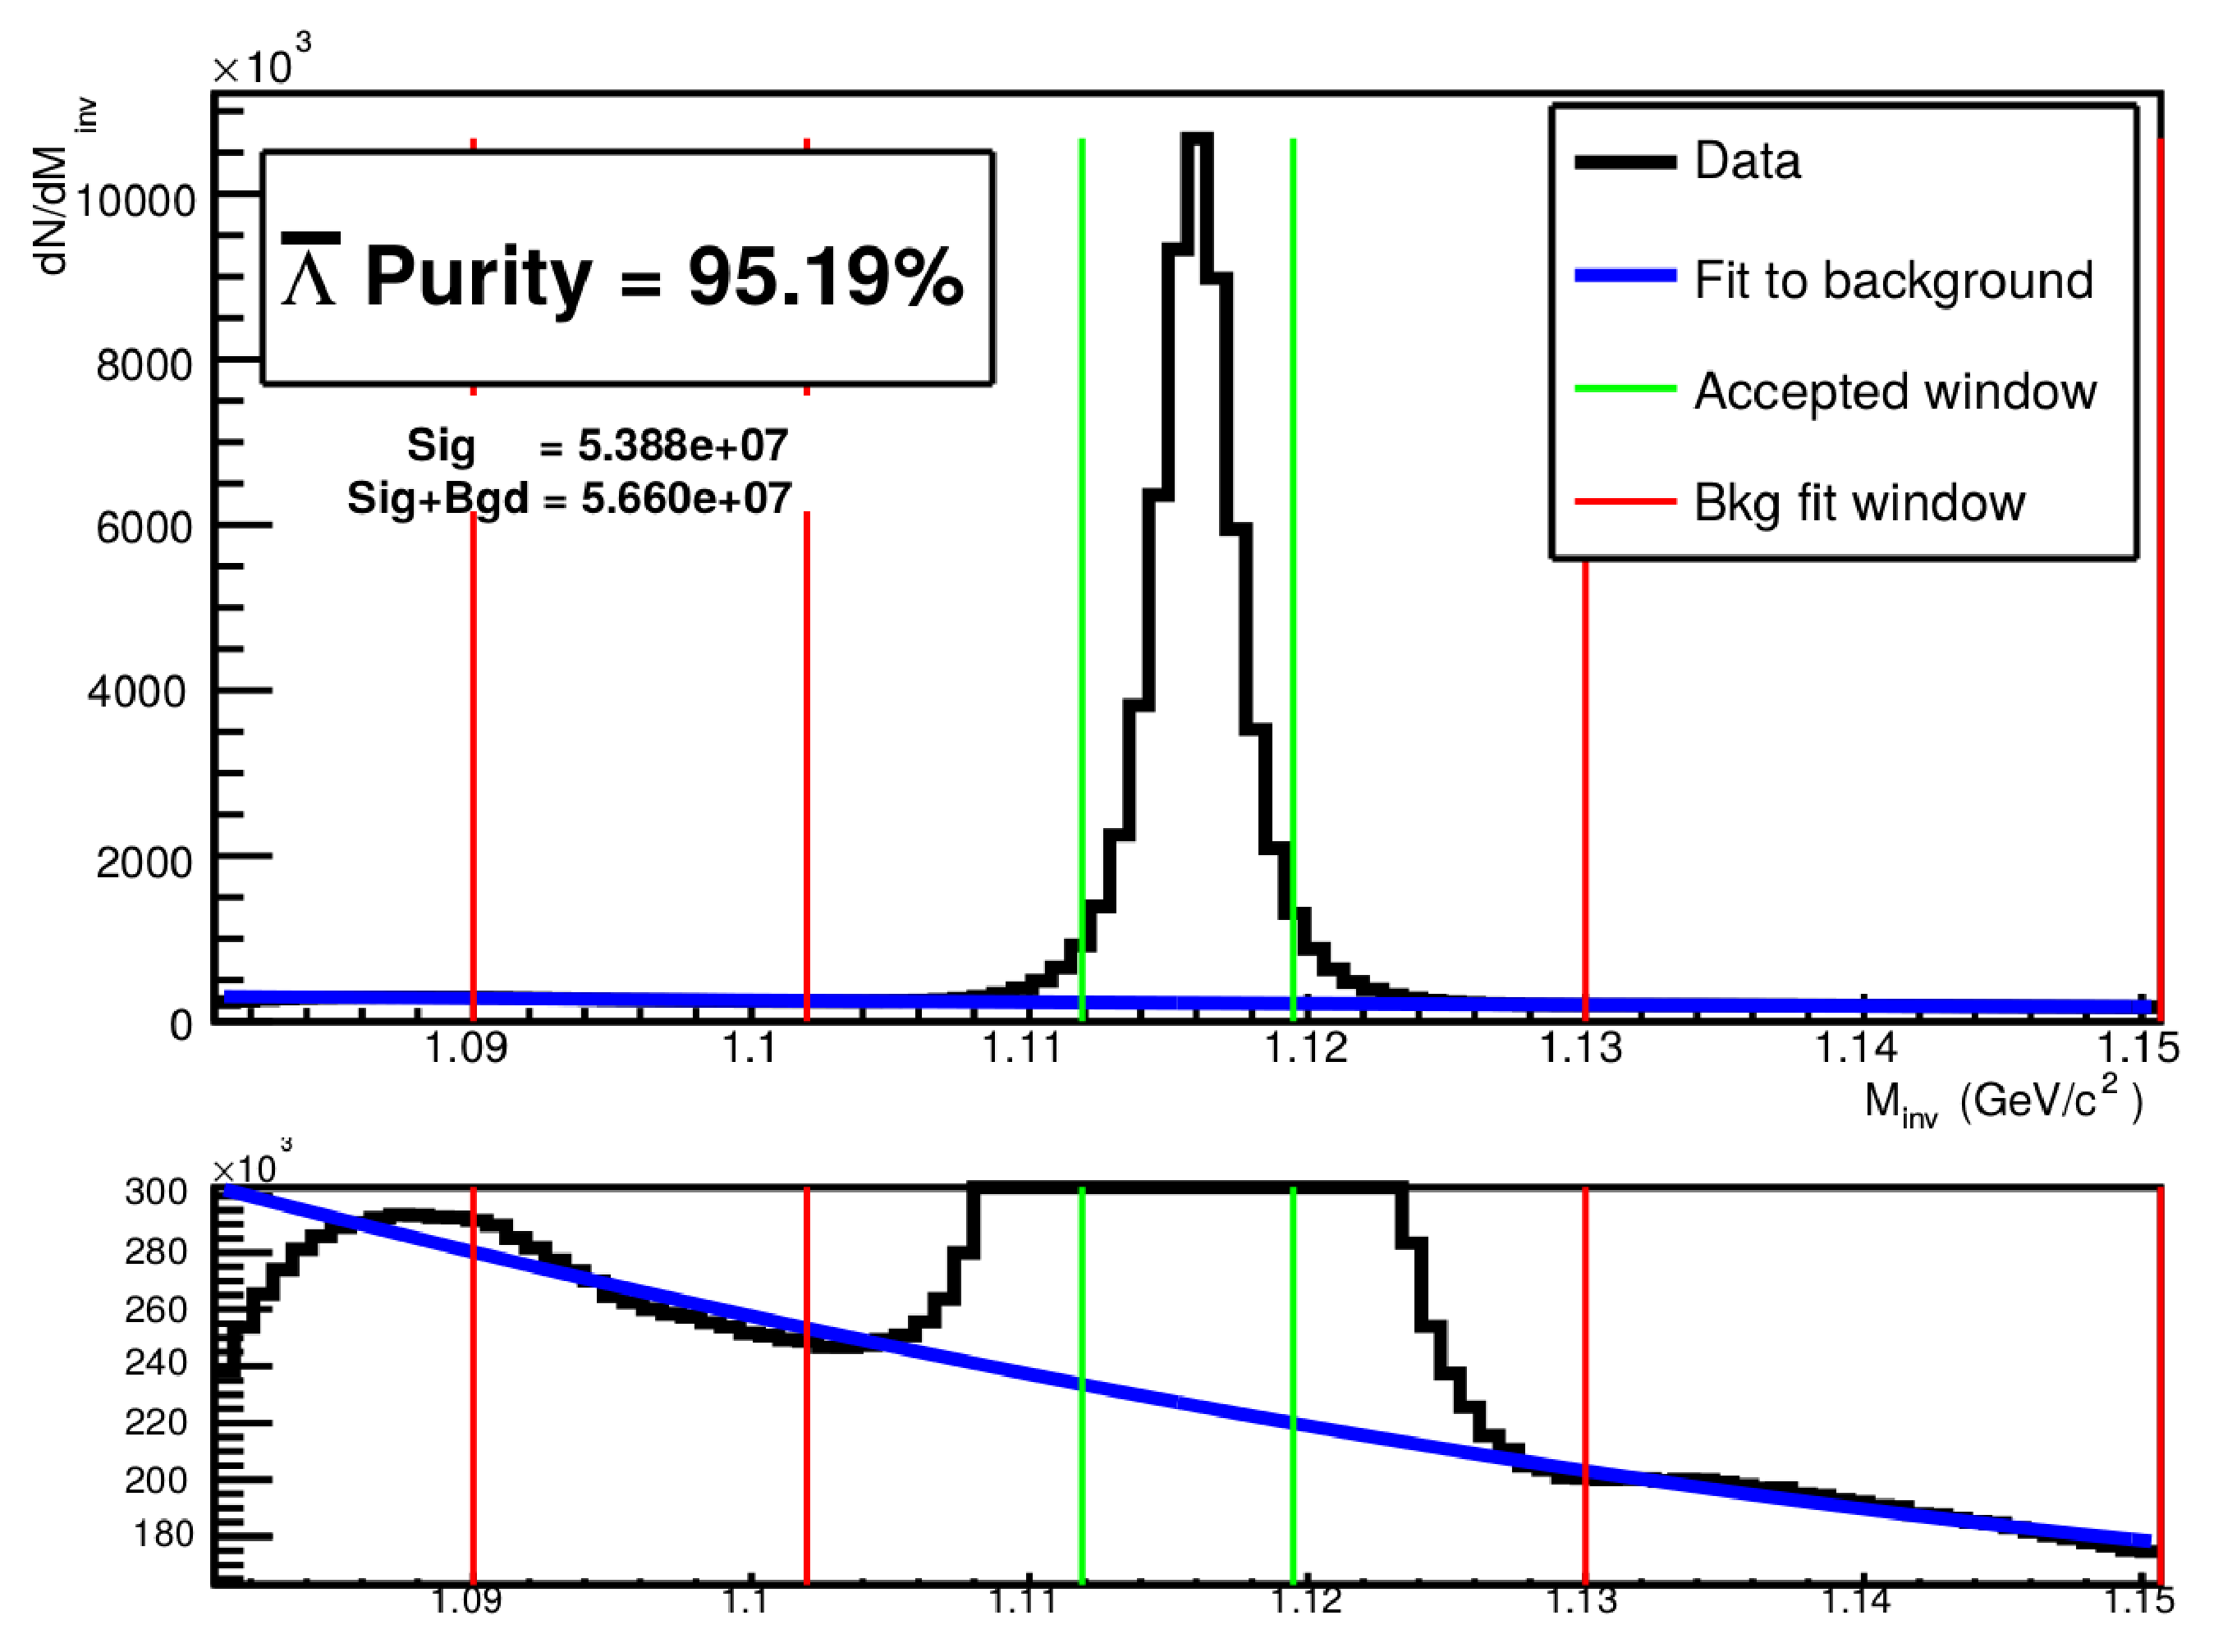
\includegraphics[width=0.49\textwidth]{3_DataSelection/Figures/ALamPurity_LamKch_0010.pdf}}
  %%----overall caption----
  \caption[\Lam and \ALam Purity]{Invariant mass (\minv) distribution for all \Lam (a) and \ALam (b) candidates immediately before the final invariant mass cut.  The bottom figures are zoomed to show the background with fit.  The vertical green lines represent the \minv cuts used in the analyses, the red vertical lines delineate the regions over which the background was fit, and the blue line shows the background fit.  These distributions are used to calculate the collection purities, Purity(\Lam) $\approx$ Purity(\ALam) $\approx$ 95\%.}
  \label{fig:cLamPurity}
\end{figure}

\end{document}